% !TEX program = pdflatex
\documentclass[11pt,a4paper]{article}

\usepackage[utf8]{inputenc}
\usepackage[T1]{fontenc}
\usepackage{lmodern}
\usepackage{geometry}
\geometry{margin=1in}
\usepackage{amsmath,amssymb}
\usepackage{siunitx}
\usepackage{graphicx}
\usepackage[font=small,labelfont=bf,labelsep=endash]{caption}
\usepackage{booktabs}
\usepackage{physics}
\usepackage{cite}
\usepackage{hyperref}
\usepackage{float}
\hypersetup{colorlinks=true,linkcolor=blue,citecolor=blue,urlcolor=blue}

\title{Design Methodology for a Hovering Disc with an Annular Air Curtain:\\
Coupled Cushion-Ground Model and Pressure-Sealing Design Procedure}
\author{Fabio Vulpi, Ph.D.}
\date{27.10.2025}

\begin{document}

\maketitle

\begin{abstract}
This work presents a physically consistent design and modelling framework for a hovering disc supported by an annular high-velocity air curtain.
The objective is to generate a central high-pressure cushion capable of sustaining an external load, while the annular jet prevents radial escape of air rather than providing vertical thrust.
The coupled model includes:
(i) an axisymmetric, low-Mach compressible core region governed by an anisotropic Darcy-Brinkman formulation, and
(ii) a momentum-based curtain sub-model acting as a pressure-sealing boundary through a mixed (Robin) condition.
A step-by-step computational procedure is defined for implementation, including the evaluation of lift, leakage, sealing index, and power.
The methodology yields a clear basis for sizing and performance assessment of air-cushion hover devices.
\end{abstract}

\begin{figure}[t]
  \centering
  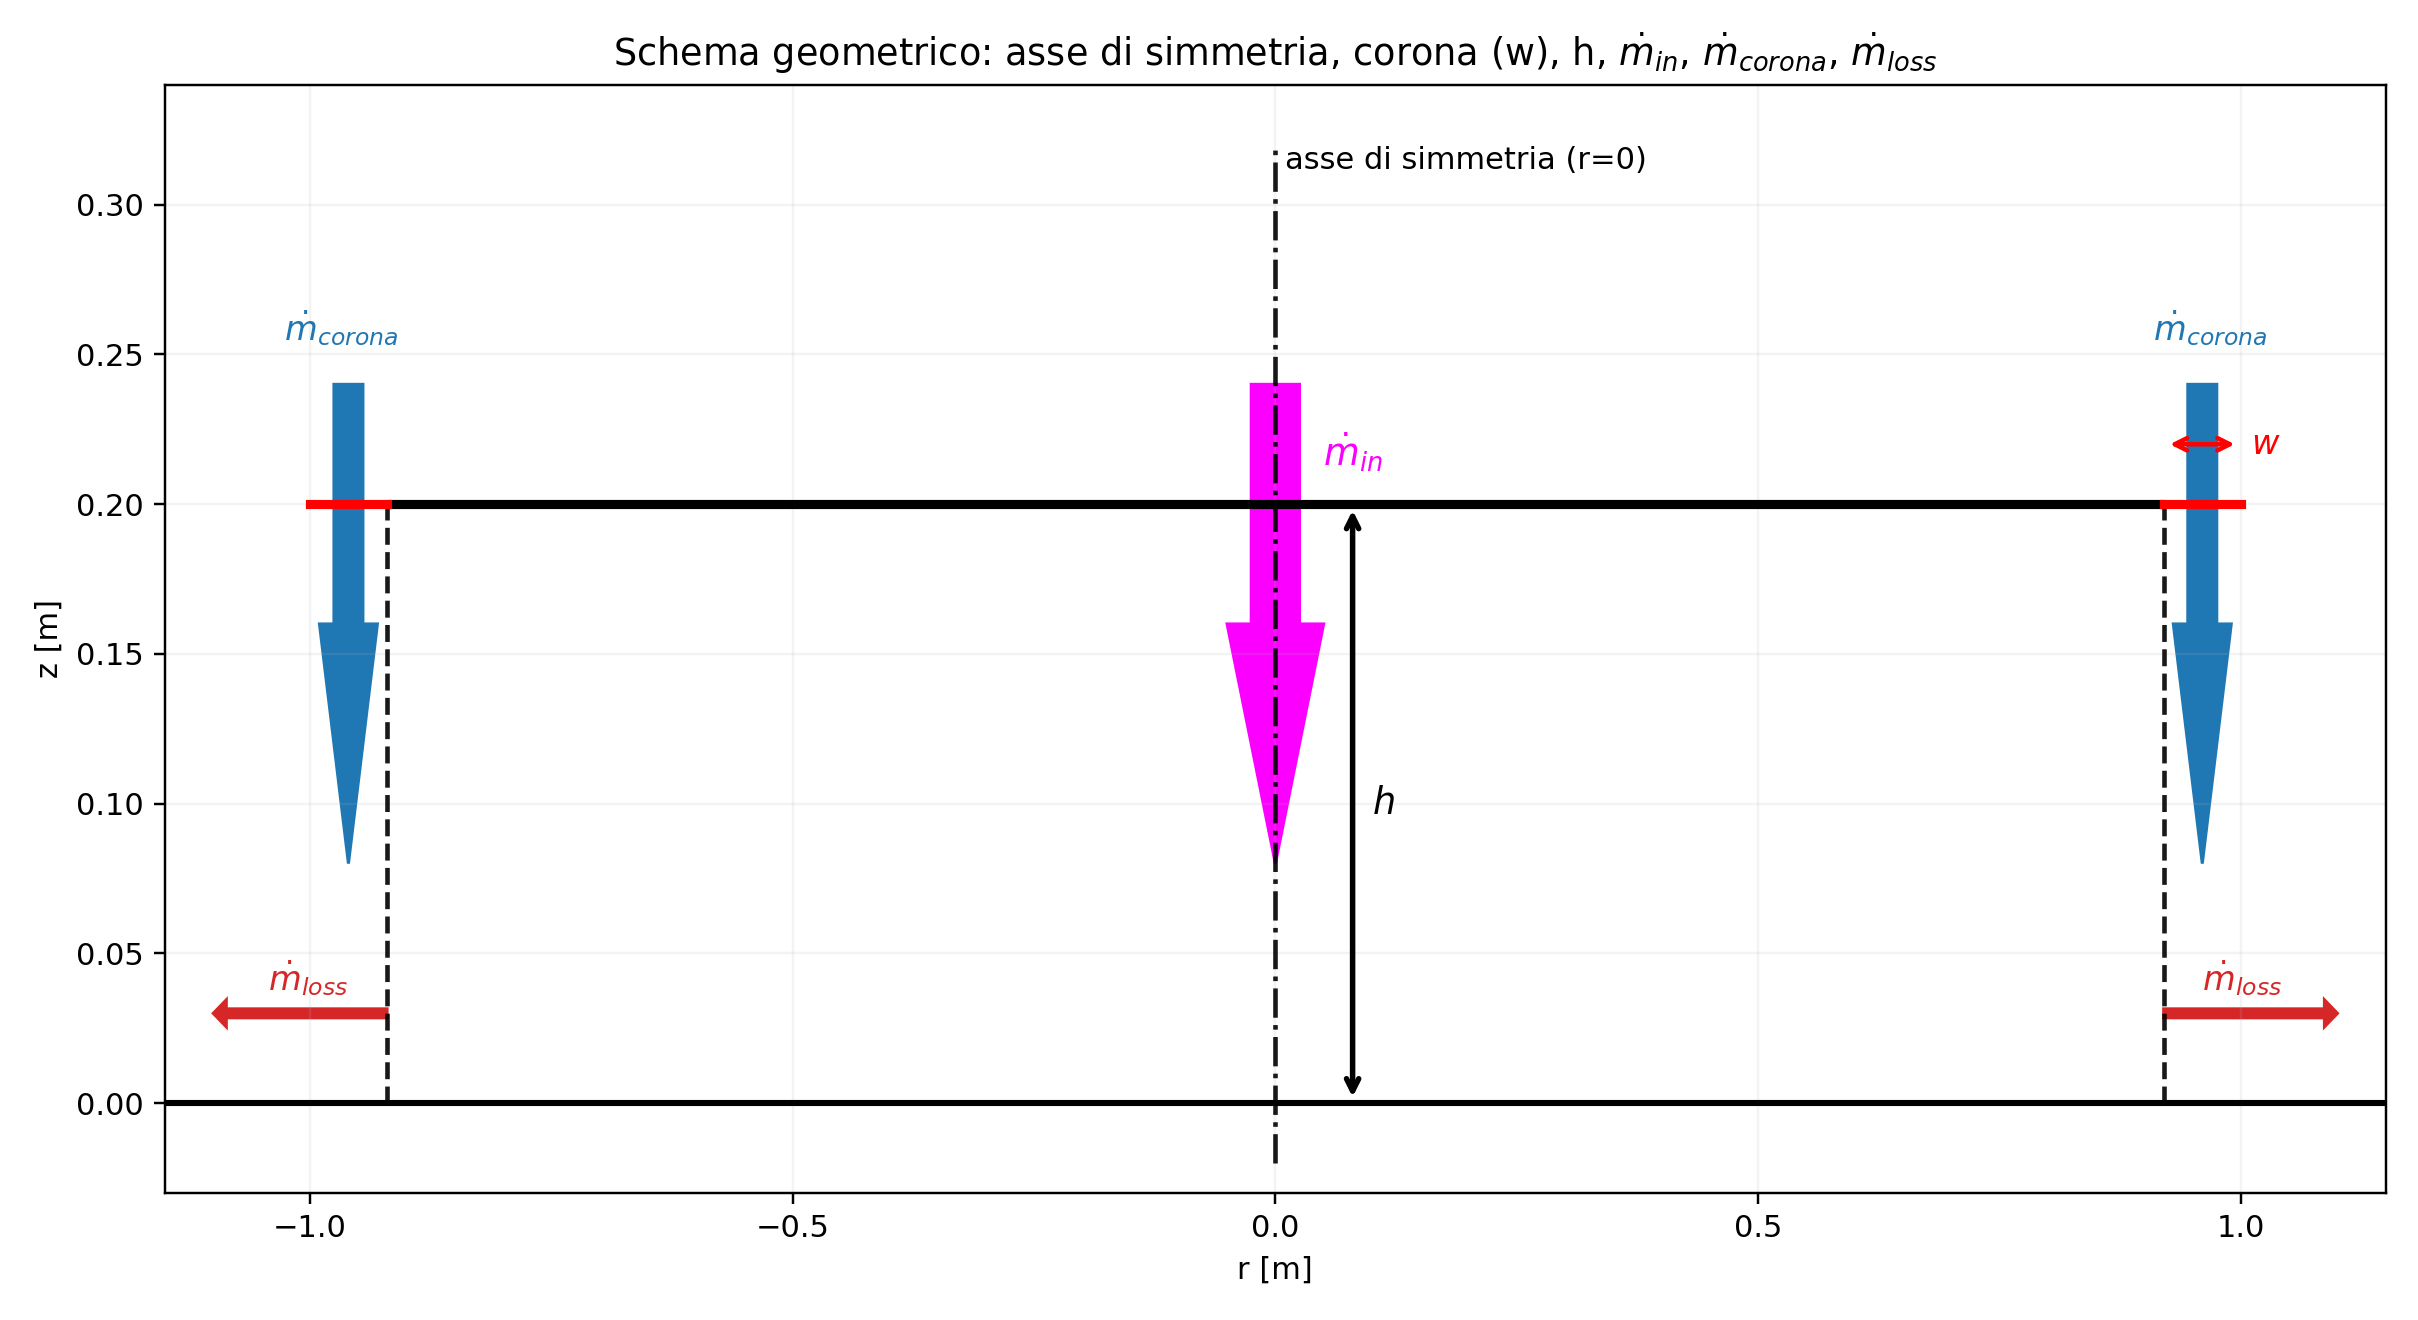
\includegraphics[width=0.95\linewidth]{../figs/schema_geometry.png}
  \caption{Schematic of the hovering disc with two concentric jets: the outer annular curtain and the central make-up flow.}
  \label{fig:geometry}
\end{figure}

\section{Geometry and Notation}
\label{sec:geometry}
The geometry follows Fig.~\ref{fig:geometry}, defining the coordinate system and characteristic dimensions:
\begin{itemize}
  \item $R_{\mathrm{tot}}$ -- total radius of the disc.
  \item $h$ -- hovering height from the ground.
  \item $h_{\mathrm{eff}}$ -- effective sealing height (characteristic of curtain recirculation).
  \item $p_0$ -- ambient pressure; $p_c=W/(\pi R_{\mathrm{tot}}^2)$ -- cushion pressure supporting the load $W$.
  \item $U_{\mathrm{out}}$, $\rho_j$ -- speed and density of the outer jet.
  \item $\mu$ -- dynamic viscosity; $R_g$ -- specific gas constant for air.
  \item $\dot{m}_{\mathrm{in}}$ -- air mass flow entering internal region.
  \item $\dot{m}_{\mathrm{out}}$ -- air mass flow of outer region.
  \item $\dot{m}_{\mathrm{loss}}$ -- air mass flow exiting internal region.
  \item $H$ -- effective curtain height (equal to $h$ in this study, representing the vertical extent over which the curtain resists leakage).
  \item $b_0$ -- slot thickness of the outer annular jet at injection; the jet centreline is located at $R^{-}=R_{\mathrm{tot}}-b_0/2$.
  \item $b(z)$ -- local width of the curtain slot as a function of $z$ (constant or weakly varying).
  \item $\varepsilon_g$ -- representative ground roughness used to define the effective sealing gap $h_{\mathrm{eff}} = h - \varepsilon_g$.
\end{itemize}

\begin{table}[h]
  \centering
  \caption{Default model parameters and empirical coefficients (nominal values are exemplary and require calibration).}
  \label{tab:model-params}
  \begin{tabular}{@{}llll@{}}
    \toprule
    Symbol & Description & Unit & Nominal value \\
    \midrule
    $\alpha_r$     & Radial permeability coefficient      & —     & (e.g.\ 0.1) \\
    $\alpha_z$     & Axial permeability coefficient       & —     & (e.g.\ 0.05) \\
    $E$            & Entrainment coefficient (wall-jet)  & —     & (e.g.\ 0.3) \\
    $C_f$          & Wall friction coefficient           & —     & (e.g.\ 0.005) \\
    $k_e$          & Wall-jet thickness growth rate      & m/m   & (e.g.\ 0.01) \\
    $K_{\rm turn}$ & Momentum loss coefficient at turning& —     & (e.g.\ 1.2) \\
    $D_{m,\min}$   & Minimum deflection modulus         & —     & (e.g.\ 0.2) \\
    \bottomrule
  \end{tabular}
\end{table}


\section{Model Overview}
\label{sec:model-overview}

The cushion region ($0\le r\le R^{-},\ 0\le z\le h$) contains the pressurized air responsible for lift generation.
Under isothermal, low–Mach conditions the mean flow obeys an \emph{anisotropic Darcy–Brinkman} law:
\begin{equation}
  u = -\frac{\kappa_r}{\mu}\,\partial_r p , \qquad
  w = -\frac{\kappa_z}{\mu}\,\partial_z p ,
  \label{eq:darcy_brinkman}
\end{equation}
where $\kappa_r=\alpha_r h^2$ and $\kappa_z=\alpha_z h^2$ represent effective permeabilities in the radial and vertical directions.
Inertia is neglected provided $Re_c=\rho U_c h/\mu\ll1$; if this limit is exceeded, a Brinkman term or RANS correction may be used.
Mass conservation and state equation read
\begin{equation}
  \frac{1}{r}\,\partial_r\!\left(r\rho u\right)+\partial_z(\rho w)=0,
  \qquad
  p=\rho R_g T_0,
\end{equation}
under the isothermal assumption $T=T_0$.
\section{Simulation Methodology}
\label{sec:simulation-method}

This section presents a clear, step-by-step procedure for simulating the coupled dynamics of the core cushion region and the outer annular curtain jet. The algorithm is designed to determine the steady pressure and velocity fields in both regions, and thereby to compute the load-carrying capacity, leakage mass flows, and power requirement of the hover system.

\subsection*{1. Domains and coupling overview}
The hover disc system is conceptually split into two interacting regions:
\begin{itemize}
  \item The \emph{core cavity}, defined by \(0 \le r \le R^{-},\;0 \le z \le h\), filled with pressurized air that supports the load and from which a peripheral leakage ring allows outflow.
  \item The \emph{outer-jet region}, comprising the annular slot at \(r=R^{-}\) through which the high-velocity curtain issues downward, impinges on the ground, and subsequently transitions into a radial wall-jet along the ground surface.
\end{itemize}
The key coupling mechanism is as follows: the outer jet impinges, creating a rim pressure distribution \(p_{\rm edge}(z)\) at the boundary \(r=R^{-}\); this rim pressure acts as a boundary condition for the core pressure field. In turn, the core pressure field determines the leakage mass flux and thus affects the required outer jet flow and velocity to maintain equilibrium.

\subsection*{2. Governing sub-problems}

\paragraph{2.1 Outer jet / curtain model}  
Given a trial outer-slot exit velocity \(U_{\rm out}\) and mass flow \(\dot m_{\rm out}\), the outer-jet sub-model now uses:
\begin{itemize}
  \item The prescribed vertical profile \(U_z(z)=U_{\mathrm{out}}\Phi(\zeta)\) with \(\Phi(1)=1\), \(\Phi(0)=0\) [Eq.~\eqref{eq:Uz_profile}], ensuring purely vertical issue at \(z=H\) and vanishing axial speed at the floor.
  \item The impingement pedestal \(\Delta p_{\mathrm{imp}}\) and turning loss \(K_{\mathrm{turn}}\) [Eq.~\eqref{eq:delta_p_imp}], setting the near-floor static build-up.
  \item The composite rim pressure \(p_{\mathrm{edge}}(z)\) with shape \(g(\zeta)\) [Eq.~\eqref{eq:pedestal_composite}] and cap \(p_0+\Delta P\).
  \item Initialization of the radial wall-jet at the turning radius \(r_t\) via \((q,m)\) conditions in Eq.~\eqref{eq:walljet_init}, then integral advancement using entrainment \(E\), friction \(C_f\) and thickness growth \(\delta'(r)=k_e\).
\end{itemize}
The curtain conductance \(C_{\mathrm{seal}}(\zeta)\) implied by the momentum part of \(p_{\mathrm{edge}}\) is used in the Robin coupling at the rim [Eq.~\eqref{eq:robin}].
\paragraph{2.2 Core cushion model}  
With \(p_{\rm edge}(z)\) now available, the core model solves:
\[
  \frac{1}{r}\,\partial_r\!\Bigl(r\,\rho\,\kappa_r\,\partial_r p\Bigr)
  + \partial_z\!\Bigl(\rho\,\kappa_z\,\partial_z p\Bigr) = 0,
  \quad
  \rho = \frac{p}{R_g\,T_\infty}, 
\]
together with the Darcy-Stokes closure:
\[
  u = -\frac{\kappa_r}{\mu}\,\partial_r p,
  \qquad
  w = -\frac{\kappa_z}{\mu}\,\partial_z p,
\]
where \(\kappa_r=\alpha_r\,h^2\), \(\kappa_z=\alpha_z\,h^2\).  
Boundary conditions:
\begin{itemize}
  \item \(\partial_r p(0,z)=0\) (axis symmetry),
  \item \(\partial_z p(r,0)=\partial_z p(r,h)=0\) (no-normal-flow at ground and disc surface),
  \item Mixed Robin sealing condition at \(r=R^{-}\):
  \[
    -\,\rho\,\kappa_r\,\partial_r p\big|_{r=R^{-}}
    = C_{\mathrm{seal}}(z)\,[\,p(R^{-},z)-p_0\,],
  \]
  where \(C_{\mathrm{seal}}(z)=\chi\,(\rho_j U_z(z)^2/\mu)(b/H)(1/D_{m,\min})\)
  includes an empirical factor \(\chi\in[0,1]\) accounting for ground roughness and non-ideal sealing.
\end{itemize}
From the computed fields \(p(r,z),\,u(r,z),\,w(r,z)\), the following integrated quantities are evaluated:
\begin{itemize}
  \item Average cushion pressure: \(\bar p_{\rm core} = \frac{1}{\pi (R^{-})^2 h}\,\displaystyle\int_0^{R^{-}}\!\int_0^h p(r,z)\,2\pi r\,dz\,dr\).
  \item Leakage mass flow through the peripheral ring: \(\dot m_{\rm leak} = \displaystyle\int_{R^{-}}^{R_{\rm tot}}\!\int_0^{h}\rho(r,z)\,u(r,z)\,dz\,dr\) (or a suitably reduced one-dimensional approximation).
  \item Lift force: \( L = \displaystyle\int_{0}^{R^{-}}\!\! (p(r,z)-p_0)\,2\pi r\,dr \approx W \).
\end{itemize}


\subsection*{3. Iterative coupling and convergence}
The overall algorithm proceeds as follows:
\begin{enumerate}
  \item Choose an initial guess for \(U_{\rm out}\), \(\dot m_{\rm out}\) and model parameters \((K_{\mathrm{turn}},D_{m,\min},E,C_f,k_e,m,\beta)\).
  \item Build the curtain profile \(U_z(z)=U_{\mathrm{out}}\Phi(\zeta)\) and the composite rim pressure \(p_{\mathrm{edge}}(z)\) [Eqs.~\eqref{eq:Uz_profile}--\eqref{eq:pedestal_composite}].
  \item Compute the sealing conductance \(C_{\mathrm{seal}}(\zeta)\) and impose the Robin coupling at \(r=R^{-}\) [Eq.~\eqref{eq:robin}]; solve the core (Darcy--Brinkman) for \(p(r,z),u,w\).
  \item Initialize and march the radial wall-jet from \(r_t\) using \((q,m)\) balances and \(\delta'(r)=k_e\) to validate the near-floor behaviour.
  \item Update \(\bar p_{\rm core}\), \(\dot m_{\rm leak}\), and lift \(L\); enforce mass balance \(\dot m_{\rm in}=\dot m_{\rm out}+\dot m_{\rm leak}\).
  \item Check convergence on load, mass balance \emph{and} a recirculation indicator (mean sign of \(u\) in a thin ring at \(r\lesssim R^{-}\)): if not converged, under-relax \(U_{\mathrm{out}}\) and the pedestal weight via \(m\) in \(g(\zeta)\), then repeat.
\end{enumerate}
Convergence tolerances are typically \(\varepsilon_L=\varepsilon_m=10^{-3}\) for load and mass, and \(\varepsilon_p=10^{-4}\) for rim-pressure updates.
The under-relaxed update of \(U_{\mathrm{out}}\) reads
\[
  U_{\mathrm{out}}^{(k+1)} = \omega\,U_{\mathrm{out}}^{(k)} + (1-\omega)\,U_{\mathrm{out}}^{\rm target}, 
  \quad 0<\omega<1,
\]
with \(\omega\simeq 0.5\); a similar under-relaxation is applied to the exponent \(m\) in \(g(\zeta)\).

\subsection*{4. Outputs and interpretation}
When the iterative loop has converged to a self-consistent state, the simulation returns:
\begin{itemize}
  \item The core fields \(p(r,z)\), \(u(r,z)\), \(w(r,z)\) and the derived out-of-plane vorticity \(\omega_\theta=\partial_r w-\partial_z u\) to visualize the near-rim recirculation cell.
  \item The rim-pressure profile \(p_{\rm edge}(z)\), the sealing conductance \(C_{\mathrm{seal}}(\zeta)\), and the wall-jet integral quantities (entrainment, wall-jet speed/thickness evolution).
  \item The mass flows \(\dot m_{\rm out}\), \(\dot m_{\rm leak}\), and effective lift \(L\), with the mass balance check \(\dot m_{\rm in}=\dot m_{\rm out}+\dot m_{\rm leak}\).
  \item The estimated outer-jet power \(\dot W_{\rm jet}\approx \dot m_{\rm out}\,\tfrac12\,U_{\rm out}^2\) corrected by turning/impingement losses.
  \item A parameter-sensitivity summary for \(h\), sealing performance and lift versus \(U_{\rm out}\), \(b_0\), \(\alpha_r\), \(\alpha_z\), \(D_{m,\min}\), \(E\), \(C_f\), \(k_e\), \(m\), \(\beta\).
\end{itemize}
Diagnostic plots should include \(U_z(z)\) and \(p_{\mathrm{edge}}(z)\) at \(r=R^{-}\), and the sign of the radial velocity in a thin ring inside the rim.
\section{Validity of Modeling Assumptions}
\label{sec:validity-of-modeling-assumptions}

\subsection{Low-Mach Compressibility}
The jets have typical velocities $U_{\mathrm{out}}\approx30$--$60\,$m/s, leading to a Mach number $Ma=U/a\approx0.1$--$0.2$ with $a\simeq343\,$m/s.
This regime justifies a \emph{low-Mach} formulation: the flow is compressible enough to exhibit pressure- and temperature-dependent density, but acoustic effects remain negligible.
Hence, the ideal-gas relation $p=\rho R_g T$ is retained, while the flow is assumed quasi-static in time.

\subsection{Thermal Uniformity and Energy Exchange}
Although the confined air experiences some compression heating, the characteristic time scales of thermal diffusion and convective mixing by the curtain are short compared to global unsteadiness.
The first-order model therefore assumes a uniform temperature $T=T_\infty$, with the understanding that future extensions may include the steady energy balance to recover small deviations of $T(r,z)$.

\subsection{Stokes--Darcy Closure}
The Stokes--Darcy model does not imply a porous medium in the literal sense.
Instead, it approximates the momentum balance of a low-Reynolds, highly dissipative, confined flow.
At low $Re=\rho U h/\mu$, the Stokes equations reduce to a linear proportionality between pressure gradient and velocity.
Replacing $\nabla^2\mathbf{u}\sim \mathbf{u}/L^2$ with an effective geometric length $L\sim h$ yields
\begin{equation}
  \mathbf{u}\approx-\frac{h^2}{\mu}\nabla p,
\end{equation}
which is mathematically equivalent to Darcy's law with an effective permeability $\kappa\sim h^2$.
The anisotropic form used here,
\begin{equation}
  \kappa_r=\alpha_r h^2,\qquad \kappa_z=\alpha_z h^2,
\end{equation}
accounts for different confinement levels in the radial and vertical directions.

\paragraph{Validity range.}
This closure is valid provided that:
\begin{itemize}
  \item the Reynolds number in the cushion $Re_c=\rho U_c h/\mu \ll 1$;
  \item pressure variations are slow and inertia negligible;
  \item the flow is quasi-steady and dominated by viscous losses and boundary friction;
  \item local turbulence and recirculation effects are absorbed into the empirical coefficients $\alpha_r,\alpha_z$.
\end{itemize}
It is particularly suited to parametric design and control studies where the detailed jet micro-structure is not resolved.


\subsection{Boundary Conditions and Curtain Coupling} \label{sec:boundaryconditions}
The outer annular jet issues \emph{downwards} and acts as an \emph{air curtain} that limits radial leakage from the cushion. 
To enforce the requested kinematics --- purely vertical at the injection plane and vanishing axial speed at the floor --- we prescribe a smooth vertical profile for the curtain axial velocity:
\begin{equation}
  U_z(z) = U_{\mathrm{out}}\,\Phi\!\left(\zeta\right), 
  \qquad \zeta=\frac{z}{H},\quad \Phi(1)=1,\ \Phi(0)=0,
  \label{eq:Uz_profile}
\end{equation}
with e.g.\ $\Phi(\zeta)=\sin^2\!\big(\tfrac{\pi}{2}\zeta\big)$ or $\Phi(\zeta)=\zeta^n$ ($n=2$--$3$) to avoid cusps. 
This choice regularizes the turning of the curtain into a radial wall-jet along the ground.

\paragraph*{Composite rim pressure with impingement pedestal.}
Upon impingement on the rigid floor, part of the curtain's kinetic energy is converted into static pressure. 
We model the impingement-induced pedestal as
\begin{equation}
  \Delta p_{\mathrm{imp}}=\xi_{\mathrm{imp}}\;\frac{1}{2}\,\rho_j\,U_{\mathrm{out}}^2,
  \qquad 
  \xi_{\mathrm{imp}}=\frac{1}{1+K_{\mathrm{turn}}},
  \label{eq:delta_p_imp}
\end{equation}
where $K_{\mathrm{turn}}$ is a turning-loss coefficient. 
The rim pressure along $r=R^{-}$ is then defined by a composite (pedestal $+$ momentum-sealing) expression, capped by the available head~$\Delta P$:
\begin{equation}
  p_{\mathrm{edge}}(z)=p_0 
  + \underbrace{\Delta p_{\mathrm{imp}}\;g(\zeta)}_{\text{impingement pedestal}}
  + \underbrace{\left(\frac{\rho_j\,U_z(z)^2\,b(z)}{H}\right)\frac{1}{D_{m,\min}}\,[1-g(\zeta)]}_{\text{momentum sealing}}
\end{equation}
with
\begin{equation}
  p_{\mathrm{edge}}(z)\le p_0+\Delta P.
  \label{eq:pedestal_composite}
\end{equation}
Here $g(\zeta)$ is a monotone increasing shape (e.g.\ $g(\zeta)=1-(1-\zeta)^m$, $m\in[2,4]$) that shifts weight from momentum sealing aloft to static build-up near the floor. 
The effective slot width may be taken as $b(z)=b_0 + s\,z$ to reflect geometric spreading.

\paragraph*{Robin sealing condition at the rim.}
Instead of prescribing $p(R^{-},z)=p_{\mathrm{edge}}(z)$ (pure Dirichlet), we impose a mixed \emph{Robin} condition that filters the exchange through the curtain, consistent with its local momentum:
\begin{equation}
  -\,\rho\,\kappa_r\,\partial_r p\big|_{r=R^{-}} 
  = C_{\mathrm{seal}}(\zeta)\,\big(p(R^{-},z)-p_0\big),
  \qquad 
  C_{\mathrm{seal}}(\zeta)=\frac{\rho_j\,U_z(z)^2}{\mu}\;\frac{b(z)}{H}\;\frac{1}{D_{m,\min}}\,[1-g(\zeta)].
  \label{eq:robin}
\end{equation}
This promotes a realistic near-floor recirculation: the curtain pushes air downward and radially outward at the ground, while the low-$\zeta$ reduction of $C_{\mathrm{seal}}$ limits leakage and bends streamlines back into the core.

\paragraph*{Wall-jet initialization at the turning radius.}
At the ground ($z=0$), in the narrow annulus where the curtain turns radially, we initialize the radial wall-jet with thickness $\delta_t$ and characteristic speed $U_c(r_t)$ at the turning radius $r_t$ by continuity of mass and momentum (including $K_{\mathrm{turn}}$):
\begin{equation}
  q(r_t)=\rho\,U_c(r_t)\,\delta_t, 
  \qquad 
  m(r_t)=\rho\,U_c(r_t)^2\,\delta_t.
  \label{eq:walljet_init}
\end{equation}
Downstream, the wall-jet integral balances are advanced with entrainment $E$ and skin-friction $C_f$ as in the base model.
\section{Non-dimensional formulation}
\label{sec:non-dimensionalization}

To improve the clarity and scalability of the numerical results, all quantities are expressed in non-dimensional form using characteristic reference scales of the system. The aim is to identify the dominant parameters governing both the pressure field in the inner core and the performance of the outer jet curtain.

\subsection{Reference quantities}

Let \(R_{\mathrm{tot}}\) denote the total radius of the levitating disk and \(h\) the nominal hovering height.  
The characteristic velocity and pressure are defined as:
\[
U_c = \frac{\kappa_r\,p_c}{\mu\,R_{\mathrm{tot}}}, 
\qquad 
p_c = \frac{W}{\pi R_{\mathrm{tot}}^2},
\]
where \(p_c\) represents the mean cushion pressure required to support the total load \(W\), \(\kappa_r\) the effective radial permeability, and \(\mu\) the dynamic viscosity of air.

Density and temperature are normalized with respect to their ambient values, \(\rho_0\) and \(T_0\), respectively.

\subsection{Dimensionless variables}

The spatial coordinates, velocity components, pressure and density are expressed as:
\[
\hat{r} = \frac{r}{R_{\mathrm{tot}}}, \qquad
\hat{z} = \frac{z}{h}, \qquad
\hat{u} = \frac{u}{U_c}, \qquad
\hat{w} = \frac{w}{U_c \, h / R_{\mathrm{tot}}}, \qquad
\hat{p} = \frac{p - p_0}{p_c}, \qquad
\hat{\rho} = \frac{\rho}{\rho_0}.
\]

Here \(p_0\) is the ambient static pressure outside the flow domain.  
The scaling of \(w\) accounts for the typical geometric aspect ratio of the system, where vertical velocities are smaller by a factor of \(h/R_{\mathrm{tot}}\).

\subsection{Governing equations in dimensionless form}

Substituting the above definitions into the Darcy-like formulation for the core region yields:
\[
\hat{u} = -\hat{\kappa}_r \frac{\partial \hat{p}}{\partial \hat{r}}, 
\qquad
\hat{w} = -\hat{\kappa}_z \frac{\partial \hat{p}}{\partial \hat{z}},
\]
\[
\frac{1}{\hat{r}} \frac{\partial}{\partial \hat{r}} 
\left( \hat{r}\, \hat{\rho} \, \hat{u} \right)
+ \frac{R_{\mathrm{tot}}}{h} \,
\frac{\partial}{\partial \hat{z}} 
\left( \hat{\rho} \, \hat{w} \right)
= 0,
\]
with the non-dimensional permeability ratios
\[
\hat{\kappa}_r = \frac{\kappa_r}{\kappa_r^0}, 
\qquad 
\hat{\kappa}_z = \frac{\kappa_z}{\kappa_r^0}, 
\]
and an anisotropy parameter
\[
S = \frac{\kappa_z}{\kappa_r} \, \frac{R_{\mathrm{tot}}}{h},
\]
which quantifies the degree of preferential flow direction within the core.

The ideal-gas equation of state becomes
\[
\hat{p} + \frac{p_0}{p_c} = \frac{\rho_0 R_g T_0}{p_c} 
\, \hat{\rho} \, \frac{T}{T_0},
\]
and, under the isothermal assumption \(T = T_0\), simplifies to 
\(\hat{p} = (p/p_c) - (p_0/p_c) = (\rho / \rho_0) - (p_0/p_c)\).

\subsection{Dimensionless groups}

The flow behaviour in the cushion region can be characterized by a small number of non-dimensional parameters:
\[
\mathrm{Re} = \frac{\rho_0 U_c R_{\mathrm{tot}}}{\mu}, \qquad
\mathrm{Ma} = \frac{U_c}{a_0}, \qquad
\Gamma = \frac{h}{R_{\mathrm{tot}}}, \qquad
S = \frac{\kappa_z}{\kappa_r} \frac{R_{\mathrm{tot}}}{h},
\]
where \(\mathrm{Re}\) and \(\mathrm{Ma}\) are the Reynolds and Mach numbers respectively, and \(\Gamma\) the geometric aspect ratio.

\subsection{Non-dimensionalization of the outer jet}

For the outer annular jet, the characteristic scales are based on its inlet velocity \(U_j\), slit width \(b\), and density \(\rho_j\).  
Dimensionless quantities are defined as:
\[
\hat{r}_j = \frac{r - R^{-}}{b}, \qquad
\hat{z}_j = \frac{z - h}{b}, \qquad
\hat{U} = \frac{U}{U_j}, \qquad
\hat{p}_j = \frac{p - p_0}{\rho_j U_j^2}.
\]
The corresponding Reynolds number and pressure coefficient are:
\[
\mathrm{Re}_j = \frac{\rho_j U_j b}{\mu}, \qquad
C_p = \frac{p - p_0}{\tfrac{1}{2}\rho_j U_j^2}.
\]
The non-dimensional entrainment and wall-friction effects are represented by:
\[
E^* = \frac{E}{U_j}, \qquad
C_f^* = C_f \frac{R_{\mathrm{tot}}}{b},
\]
while the turn-loss and minimum-momentum-deflection parameters are introduced as:
\[
K_{\mathrm{turn}}^* = \frac{K_{\mathrm{turn}}}{\rho_j U_j^2}, \qquad
D_{m,\min}^* = D_{m,\min}.
\]
This formulation allows direct comparison between the dynamic capacity of the jet
(\(\rho_j U_j^2 b / H\)) and the dimensionless cushion pressure \(\hat{p}_c = p_c / (\rho_j U_j^2)\),
thereby linking the jet operating point with the pressure sustained in the core.

\subsection{Interpretation}

With this formulation:
- quantities inside the core scale naturally with the load \(W\), geometry \((R_{\mathrm{tot}},h)\), and permeability ratios;
- quantities related to the outer jet scale with its momentum flux and geometric confinement parameters \((b,H)\);
- the coupling condition at the interface \(r = R^{-}\) can be expressed consistently as a non-dimensional pressure continuity constraint:
  \[
  \hat{p}_{\mathrm{edge}} = 
  \min\left( 
      \frac{\Delta P}{p_c}, 
      \frac{\rho_j U_j^2 b}{H D_{m,\min} p_c}
  \right),
  \]
  ensuring that both regions share a unified, dimensionless reference frame.



\section{Simulation Outputs}
\label{sec:simulation-outputs}

The results produced from the model are shown in this section.

\begin{figure}[H]
  \centering
  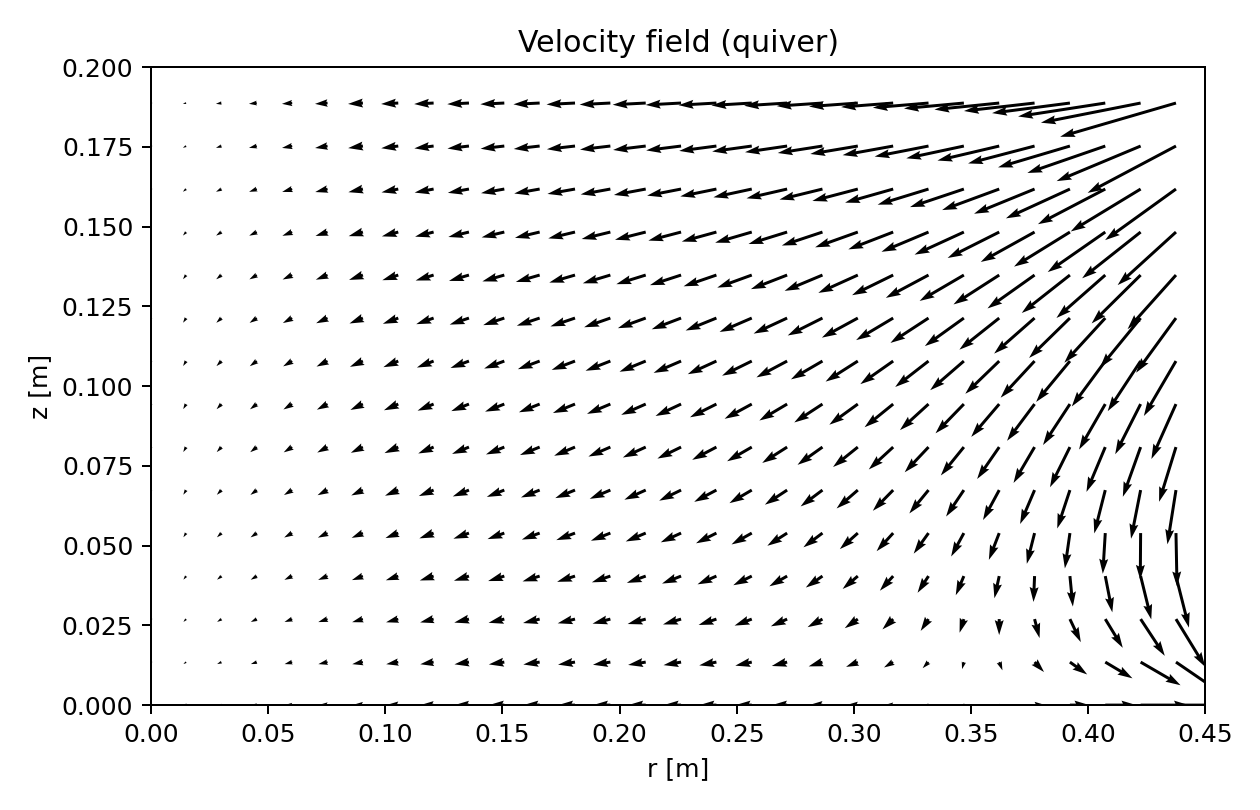
\includegraphics[width=0.95\linewidth]{../figs/quiver_velocity.png}
  \caption{Non-dimensional velocity field (quiver).
Vectors show $(\hat u,\,S\hat w)$ for isotropic visual scaling; the pattern reflects the rim-imposed sealing pressure from the downward curtain.}
  \label{fig:quiver}
\end{figure}
\begin{figure}[H]
  \centering
  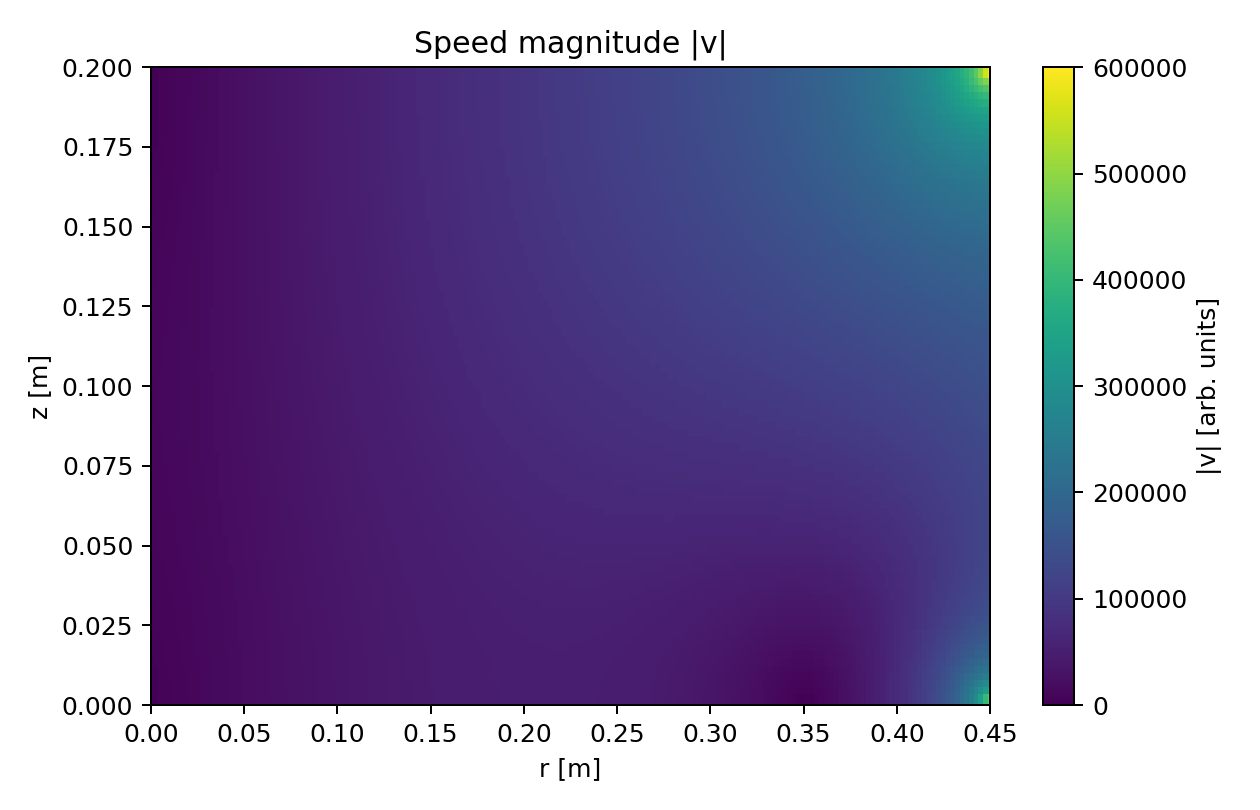
\includegraphics[width=0.95\linewidth]{../figs/cmap_speed.png}
  \caption{Colormap of the non-dimensional isotropic speed magnitude $\hat V_{\mathrm{iso}}=\sqrt{\hat u^{\,2}+S^{2}\hat w^{\,2}}$.}
  \label{fig:cmap_speed}
\end{figure}
\begin{figure}[H]
  \centering
  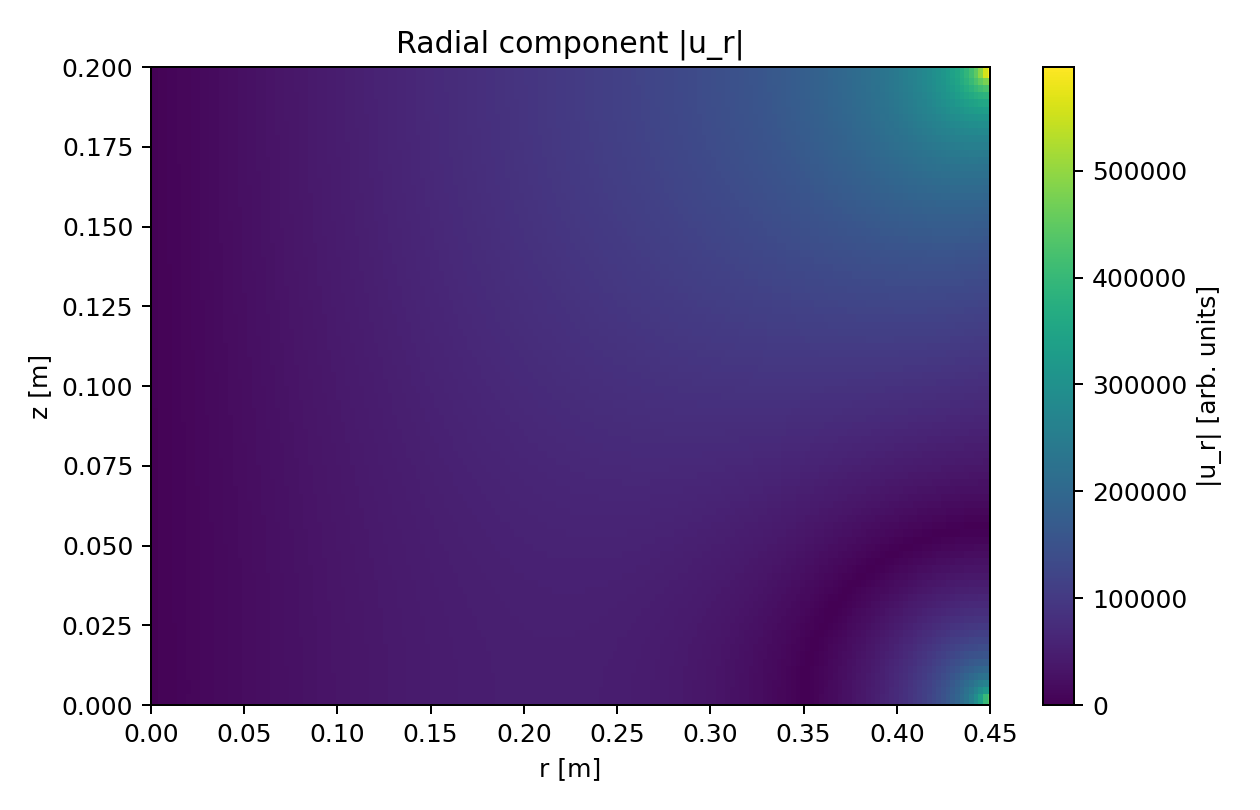
\includegraphics[width=0.95\linewidth]{../figs/cmap_ur.png}
  \caption{Colormap of the non-dimensional radial component magnitude $|\hat u|$.}
  \label{fig:cmap_ur}
\end{figure}
\begin{figure}[H]
  \centering
  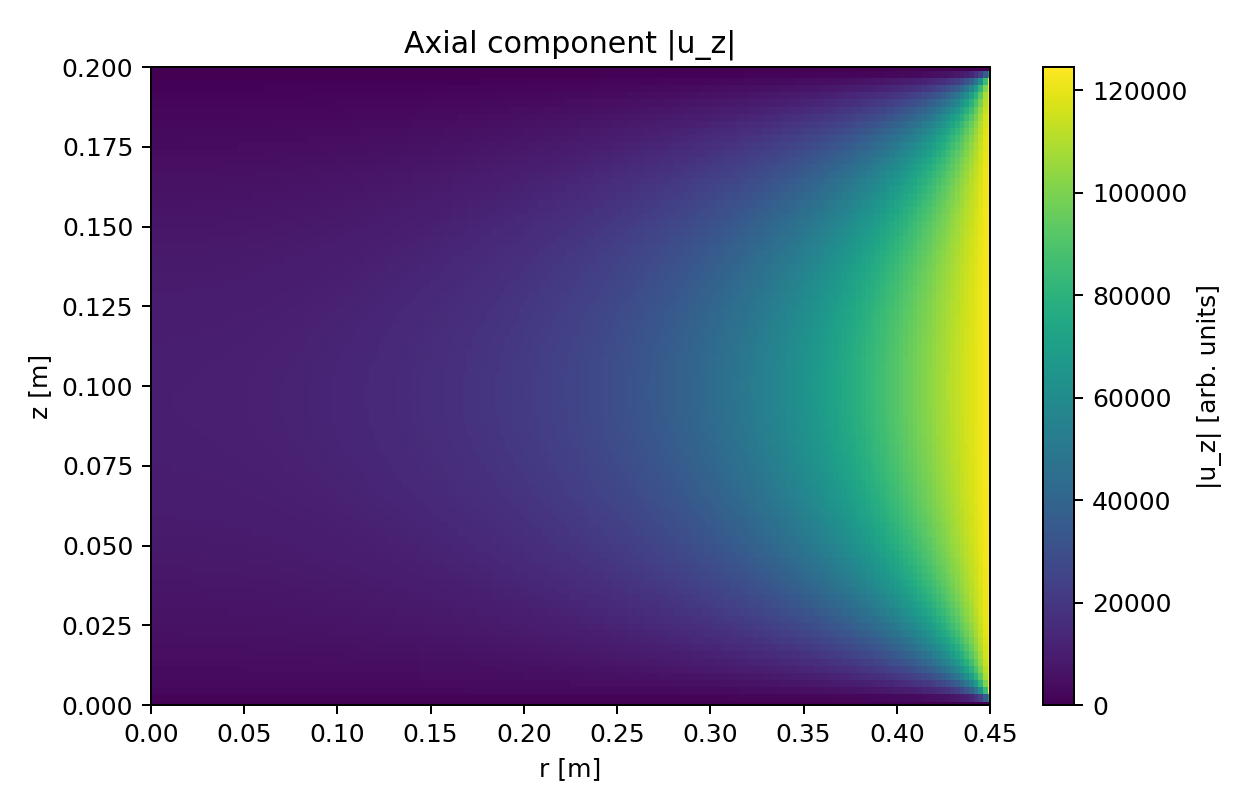
\includegraphics[width=0.95\linewidth]{../figs/cmap_uz.png}
  \caption{Colormap of the non-dimensional axial component magnitude $|\hat w|$.}
  \label{fig:cmap_uz}
\end{figure}
\begin{figure}[H]
  \centering
  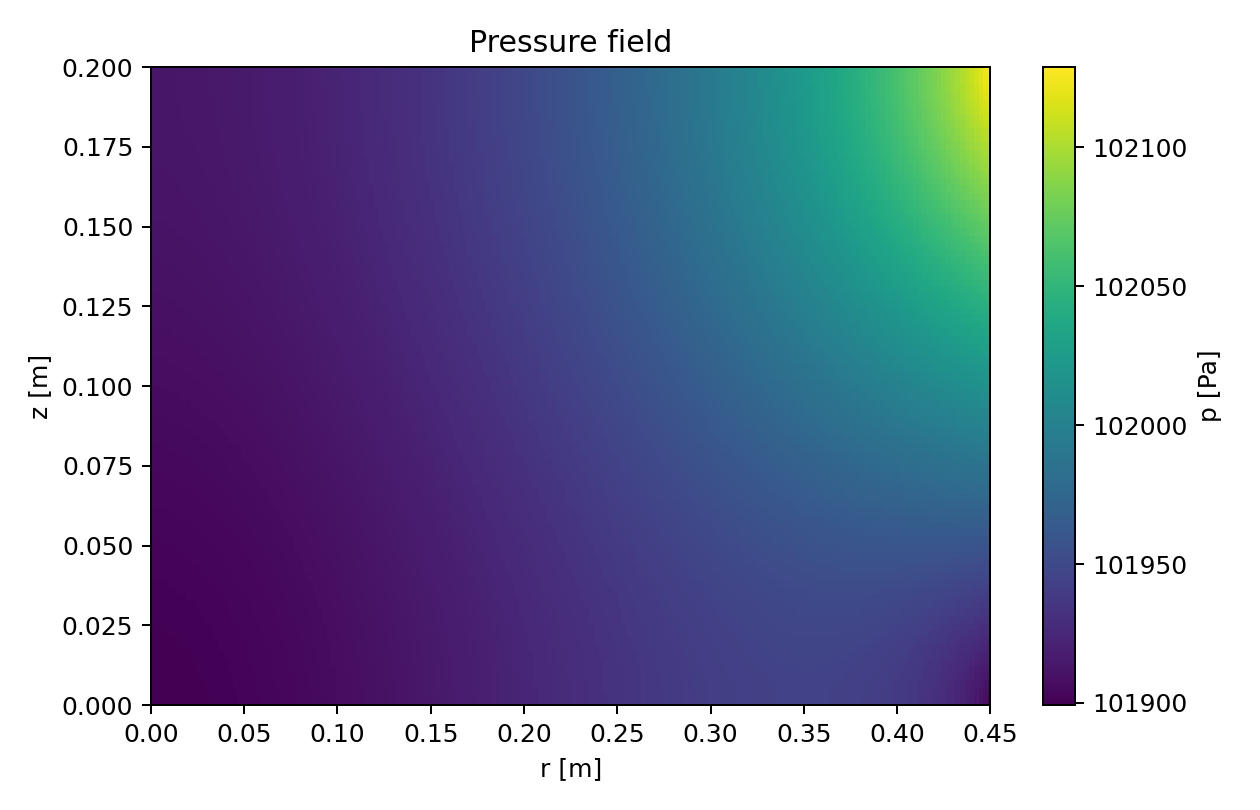
\includegraphics[width=0.95\linewidth]{../figs/cmap_pressure.png}
  \caption{Colormap of the non-dimensional pressure $\hat p$.}
  \label{fig:cmap_p}
\end{figure}

\paragraph{Performance and stability analysis.}
From the converged solutions the lift–height characteristic $L(h)$ is evaluated to assess static stability.
A stable hovering point satisfies $dL/dh < 0$ in the neighbourhood of the nominal gap.
The required jet power is estimated as
\[
  \dot W_{\mathrm{jet}} = \frac{1}{2}\dot m_{\mathrm{out}} U_{\mathrm{out}}^2 /(1+K_{\mathrm{turn}}),
\]
and the non-dimensional sealing and leakage indices are
\[
  \Pi_{\mathrm{seal}} = \frac{\rho_j U_{\mathrm{out}}^2 b}{H p_c},
  \qquad
  \Pi_{\mathrm{leak}} = \frac{\dot m_{\mathrm{leak}}}{\rho_0 U_{\mathrm{out}} 2\pi R^{-} b}.
\]
These provide quick performance metrics for design optimization.

\section*{Design Procedure Summary}
\begin{enumerate}
  \item Specify $W$, $R$, $h$, and air properties $(\rho_0,\mu,T_0)$.
  \item Compute target cushion pressure $p_c = W/(\pi R^2)$.
  \item Choose sealing index $\Sigma_{\min}\!\in[3,5]$ and estimate
        $U_{\mathrm{out}}=\sqrt{\Sigma_{\min} H p_c / (\rho_j b)}$.
  \item Evaluate $Ma$, $Re_j$ and adjust $(b,H)$ for $Ma<0.3$, $Re_j>2000$.
  \item Iterate the coupled solver until $|L-W|/W<10^{-3}$ and mass balance error $<10^{-3}$.
  \item Output: $L(h)$ curve, $\Pi_{\mathrm{seal}}$, $\Pi_{\mathrm{leak}}$, $\dot W_{\mathrm{jet}}$.
\end{enumerate}

\section{Model Limitations and Planned Extensions}
\label{sec:model-limitations-and-planned-extensions}

The present formulation uses the Darcy–Brinkman reduction as an effective description of the viscous core.
Coefficients $\alpha_r$ and $\alpha_z$ should be calibrated from axisymmetric CFD or experiments.
The secondary make-up flow is lumped into the global mass balance rather than as a local inlet.
Thermal effects are neglected ($T=T_\infty$) and Mach numbers remain below 0.3.
Future extensions will introduce a steady energy equation, refined wall-jet correlations and the automated lift-matching loop.

\paragraph{Appendix: minimal rationale for the composite rim pressure.}
Consider a control volume hugging the rim over height $h$ and thickness $O(b)$.
A downward slot jet of density $\rho_j$ and speed $U_{\mathrm{out}}$ is deflected
into a radial wall-jet of speed $U_r(z)$ near the floor. A crude momentum balance
suggests a static build-up $\Delta p_{\mathrm{stat}}\sim \rho_j U_{\mathrm{out}}^2
\,\mathcal{O}(1)$ concentrated near $\zeta\!\to\!0$, while the resistance to
cross-flow (sealing) scales with the jet momentum flux impinging near the slot,
$\Delta p_{\mathrm{seal}}\sim \rho_j U_{\mathrm{out}}^2\,\mathcal{O}(1)$ for
$\zeta\!\to\!1$. The composite form
$\rho_j U_{\mathrm{out}}^2\,[\,C_p(1-\zeta)^n + C_s \zeta^m\,]$ is thus a
first-order surrogate capturing both effects with two tunable, dimensionless
coefficients $(C_p,C_s)$ and mild shape exponents $(m,n)$.

\paragraph{On the choice of $D_{m,\min}$.}
We take $D_{m,\min}$ from air-curtain literature (order $10^{-1}$) as a design parameter; in absence of calibration, $D_{m,\min}=0.2$ provides a conservative default.
Sensitivity to this parameter is reported without altering the solver or figures.

\section{Nomenclature}
\label{sec:nomenclature}

\begin{tabular}{@{}ll@{}}
\toprule
Symbol & Description \\ \midrule
$R_{\mathrm{tot}}$ & Total radius of the disc \\
$R^{-}$ & Inner radius of the leakage ring (centreline of jet slot, $R^{-}=R_{\mathrm{tot}}-b_0/2$) \\
$h$ & Hovering height (disc--ground gap) \\
$h_{\mathrm{eff}}$ & Effective sealing height at rim \\
$b_0$ & Slot thickness at injection (plane jet width) \\
$b(z)$ -- effective local width of the curtain slot or equivalent jet region as a function of $z$ \\
$U_{\mathrm{out}}$ & Outer jet velocity \\
$\rho_j$ & Density of outer jet \\
$\rho$ & Density in the core region \\
$p,p_0,p_c$ & Local, ambient, and cushion pressures \\
$T,T_\infty$ & Local and ambient temperatures \\
$\mu$ & Dynamic viscosity of air \\
$R_g$ & Specific gas constant of air \\
$W$ & Payload supported by cushion \\
$\kappa_r,\kappa_z$ & Effective permeabilities (radial/axial) \\
$\alpha_r,\alpha_z$ & Dimensionless permeability coefficients \\
$u,w$ & Velocity components (radial, vertical) \\
$\Delta p$ & Rim pressure increment \\
$\Pi_{\mathrm{edge}}$ & Dimensionless rim pressure amplitude \\
$\mathcal{A}$ & Permeability anisotropy parameter \\
$\hat r,\hat z,\hat p$ & Dimensionless coordinates and pressure \\
$\hat u,\hat w$ & Dimensionless velocity components \\
$S$ & Velocity anisotropy ratio $S=(\alpha_z/\alpha_r)(R_{\mathrm{tot}}/h)$ \\ $D_m$ & Deflection modulus (momentum index) $\rho U_0^2 b_0/(\Delta P\,H)$ \\
$D_{m,\min}$ & Minimum deflection modulus for sealing \\
$H$ & Effective curtain height \\
$s$ & Jet spreading parameter ($\approx0.06$--$0.09$) \\
$\Delta P_{\max}$ & Maximum sustainable pressure difference \\
$q(r)$ & Mass flow per unit circumference in wall-jet model \\
$m(r)$ & Momentum flux per unit circumference in wall-jet model \\
$\delta_t$ & Wall-jet thickness at turning radius $r_t$ \\
$r_t$ & Effective turning radius of the outer jet on the ground \\
$U_c(r)$ & Local characteristic velocity of the wall-jet at radius $r$\\
\bottomrule
\end{tabular}

% =====================================================

% --- Added notation for outer-jet seal model ---
\paragraph{Additional symbols.}
\begin{tabular}{ll}
\(r_t\) & effective turning radius of the outer jet \\
\(U_{\mathrm{out}}\) & injection speed of the outer (vertical) jet \\
\(A_{\mathrm{slot}}\) & outlet area of the outer jet \\
\(K_{\mathrm{turn}}\) & momentum loss coefficient at turning (impingement) \\
\(\delta\), \(\delta_t\), \(\delta_s\) & wall-jet thickness (generic / at \(r_t\) / at \(r_-\)) \\
\(U_c(r)\) & characteristic wall-jet speed \\
\(q(r)\), \(m(r)\) & mass and momentum per unit circumference \\
\(E\) & entrainment coefficient \\
\(C_f\) & wall friction coefficient, \(C_f=C_{f0} Re_\delta^{-1/5}\) \\
\(k_e\) & wall-jet thickness growth rate \\
\(w_s\) & seal strip width, \(w_s=\lambda\,\delta_s\) \\
\(\delta_p\) & effective thickness for pressure work in the seal strip \\
\(\Delta p\) & pressure jump between core and ambient
\end{tabular}


\end{document}